\documentclass{beamer}
\usepackage[french]{babel}
\usepackage[utf8]{inputenc}
\usepackage[T1]{fontenc}
\usepackage{lmodern}
\usepackage{amssymb}
\usepackage{amsmath}
\usepackage{graphics}


%mettre du code avec \begin{lstlisting}
\usepackage{listings}
\lstset{
  basicstyle=\fontsize{7}{9}\selectfont\ttfamily,
  breaklines=true,
  tabsize=2,
  inputencoding=utf8,
  extendedchars=true,
  literate={\ \ }{{\ }}1 {á}{{\'a}}1 {ã}{{\~a}}1 {é}{{\'e}}1,
}


%taper \bo S pour taper un S calligraphié
\newcommand{\bo}[1]{\mathcal #1}

%opérateurs
\newcommand{\po}{\mathrm{o}} %composition
\newcommand{\go}{\mathrm{O}}
\newcommand{\inter}{\cap}
\newcommand{\union}{\cup}

%inégalités
\renewcommand{\leq}{\leqslant} % <=
\renewcommand{\geq}{\geqslant} % >=

%implications
\newcommand{\ssi}{\Leftrightarrow }
\newcommand{\sssi}{\Longleftrightarrow }
\newcommand{\imp}{\Rightarrow }

%ensembles de nombres
\newcommand{\N}{\mathbb N }
\newcommand{\Z}{\mathbb Z }
\newcommand{\D}{\mathbb D }
\newcommand{\Q}{\mathbb Q }
\newcommand{\R}{\mathbb R }
\newcommand{\C}{\mathbb C }
\newcommand{\K}{\mathbb K }


%analyse
\renewcommand{\d}{\text{d}} %dx/dt machin
\newcommand{\pr}{^{\prime}} %primes de dérivation
\newcommand{\prr}{^{\prime\prime}}
\newcommand{\prn}[1]{^{(#1)}}


%fonctions
\newcommand{\asin}{\text{Arcsin} }
\newcommand{\acos}{\text{Arccos} }
\newcommand{\atan}{\text{Arctan} }
\newcommand{\sh}{\text{sh} }
\newcommand{\ch}{\text{ch} }
\newcommand{\e}[1]{\left\lfloor#1\right\rfloor} %partie entière


\usepackage{minted}

\graphicspath{{figs/}}
\usefonttheme[onlymath]{serif}

\title{Modélisation de la diffusion thermique.}
\author{Josselin SCOUARNEC}
\date{Mai 2021}

\begin{document}

    \maketitle


    \begin{frame}
    \frametitle{Présentation de l'expérience}

    \begin{center}
    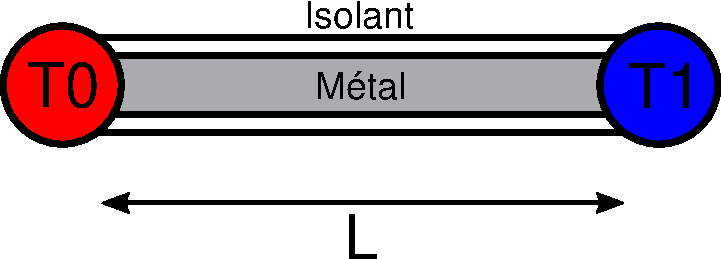
\includegraphics[width=0.6\linewidth]{figs/schem.pdf}
    \end{center}

    On note $T(x, t)$ la température de la barre à la position $x$ et à l'instant $t$. La température vérifie l'équation suivante :

    $$\frac{\partial T}{\partial t } = k\frac{\partial^2 T}{\partial x^2 }$$

    La variation de température en $x$ par rapport à $t$ est proportionnelle à une certaine variation de température par rapport à $x$. Rq : elle est nulle pour un profil linéaire.



    \end{frame}

    \begin{frame}
    \frametitle{Discrétisation du problème}

    On approxime les variations par des taux d'accroissement. Intuitivement la variation d'ordre $2$ est la variation de la variation. On remplace :

    \medskip

    $$\frac{\partial T}{\partial t } \longrightarrow \frac{T(t + \Delta T) - T(t)}{\Delta t }$$


   	$$\frac{\partial^2 T}{\partial x^2} \longrightarrow \frac{(T(x + \Delta x)-T(x)) - (T(x-\Delta x) -T(x))}{\Delta x ^2 }$$

    \bigskip

    L'équation devient :

    $$\small\boxed{T(x, t + \Delta t) = T(x, t) + k \Delta t \frac{T(x+ \Delta x, t) + T(x-\Delta x, t) -2T(x, t)}{\Delta x ^2 }}$$


    \end{frame}


    \begin{frame}
    \frametitle{Normalisation et conditions limites}


    On pose $\theta(x,t) = \frac{T(x,t) -T_1}{T_0 - T_1}$ la température normalisée,
    ainsi les paramètres $T_0$ et $T_1$ n'interviennent plus.

    \medskip

    On a les conditions suivantes sur les extrémités de la barre : $\theta(0, t) = 1$ et $\theta(L, t) = 0$.

    \medskip

    Comme $T = \theta(T_0 - T_1) + T_1$ on trouve une équation très similaire :

    $$\boxed{\theta(x, t + \Delta t) = \theta(x, t) + \Delta t \frac{\theta(x+ \Delta x, t) + \theta(x-\Delta x, t) -2\theta(x, t)}{\Delta x ^2 }}$$

    \medskip

    On peut poser $k = 1$ et $L = 1$.


    \end{frame}


    \begin{frame}
    \frametitle{Résolution numérique}

    À partir des paramètres $L$, $t_f$, $\Delta x$ et $\Delta t$, on défini un tableau que l'on va remplir avec les valeurs que l'on va calculer. On peut déjà renseigner les conditions initiales et limites.

    \begin{center}
	    \begin{tabular}{ |c|c|c|c|c|c| }
	     \hline
	     $x, t$ & $t_0$ & $t_1$ & $t_2$ & ... & $t_f$ \\
	     \hline
	     $0$   & $\theta_{0,0}$ & $1$ & $1$ &  & $1$\\
	     $x_2$ & $\theta_{1,0}$ & $\theta_{1,1}$ & $\theta_{1,2}$ &  & $\theta_{1,f}$\\
	     $x_3$ & $\theta_{2,0}$ & $\theta_{2,1}$ & $\theta_{2,2}$ &  & $\theta_{2,f}$\\
	     ... & ... & ... & ... &  & ... \\
	     $x_n = L$ &   $\theta_{n,0}$ & $0$ & $0$ &  & $0$\\
	     \hline
	    \end{tabular}
  	\end{center}

  	Chaque colonne décrit un instant et peut être calculée à partir de la colonne précédente en appliquant la formule de récurrence à chaque valeur.

    \end{frame}


	\begin{frame}[fragile]
    \frametitle{Implémentation}
    \framesubtitle{Initialisation}

\begin{minted}[fontsize=\tiny]{Python}
import numpy as np
import matplotlib.pyplot as plt

#constantes
L  = 10.0
dx = 0.1
tf = 50.0
dt = 0.001

#vérification humaine si le pas est trop grand
if (delta := dt/(dx*dx) ) > 0.1 :
    input(f'Delta = {delta}, continuer ?')


n_x = int(L/dx)  #nombre de valeurs de X
n_t = int(tf/dt) #nombre de valeurs de t

thet = np.zeros((n_x, n_t)) #matrice de résultats

thet[:, 0].fill(0) #conditions initiales
thet[0].fill(1)    #conditions limites
thet[-1].fill(0)

#différentielle
d_theth = lambda x,t : (thet[x+1][t-1] + thet[x-1][t-1] - 2*thet[x][t-1])/(dx*dx)


\end{minted}


    \end{frame}



    \begin{frame}[fragile]
    \frametitle{Implémentation}
    \framesubtitle{Exécution}

\begin{minted}[fontsize=\tiny]{Python}
#argument des ranges : ignorer les conditions initiales/limites
#évite les erreurs d'indices

for t in range(1, n_t) :

    #traité comme un système de n_x équations
    for x in range(1, n_x-1) :
        thet[x][t] = thet[x][t-1] + d_theth(x,t) * dt

    #pourcentage de complétion
    print(f'Simulation {round(t/n_t*100)}%', end='\r')

print("\nOK")


#affichage histogramme 2D
plt.imshow(thet, extent=(0, tf, 0, L), cmap='inferno', interpolation='nearest', aspect='auto')
cb = plt.colorbar()

#titre et légendes
cb.set_label('Température')
plt.xlabel('Temps')
plt.ylabel('Position')
plt.title('Évolution de la température dans une barre métallique')

plt.show()
\end{minted}


    \end{frame}


    \begin{frame}
    \frametitle{Résultats}
    \framesubtitle{Profil initial uniforme en $0$}

    \begin{center}
    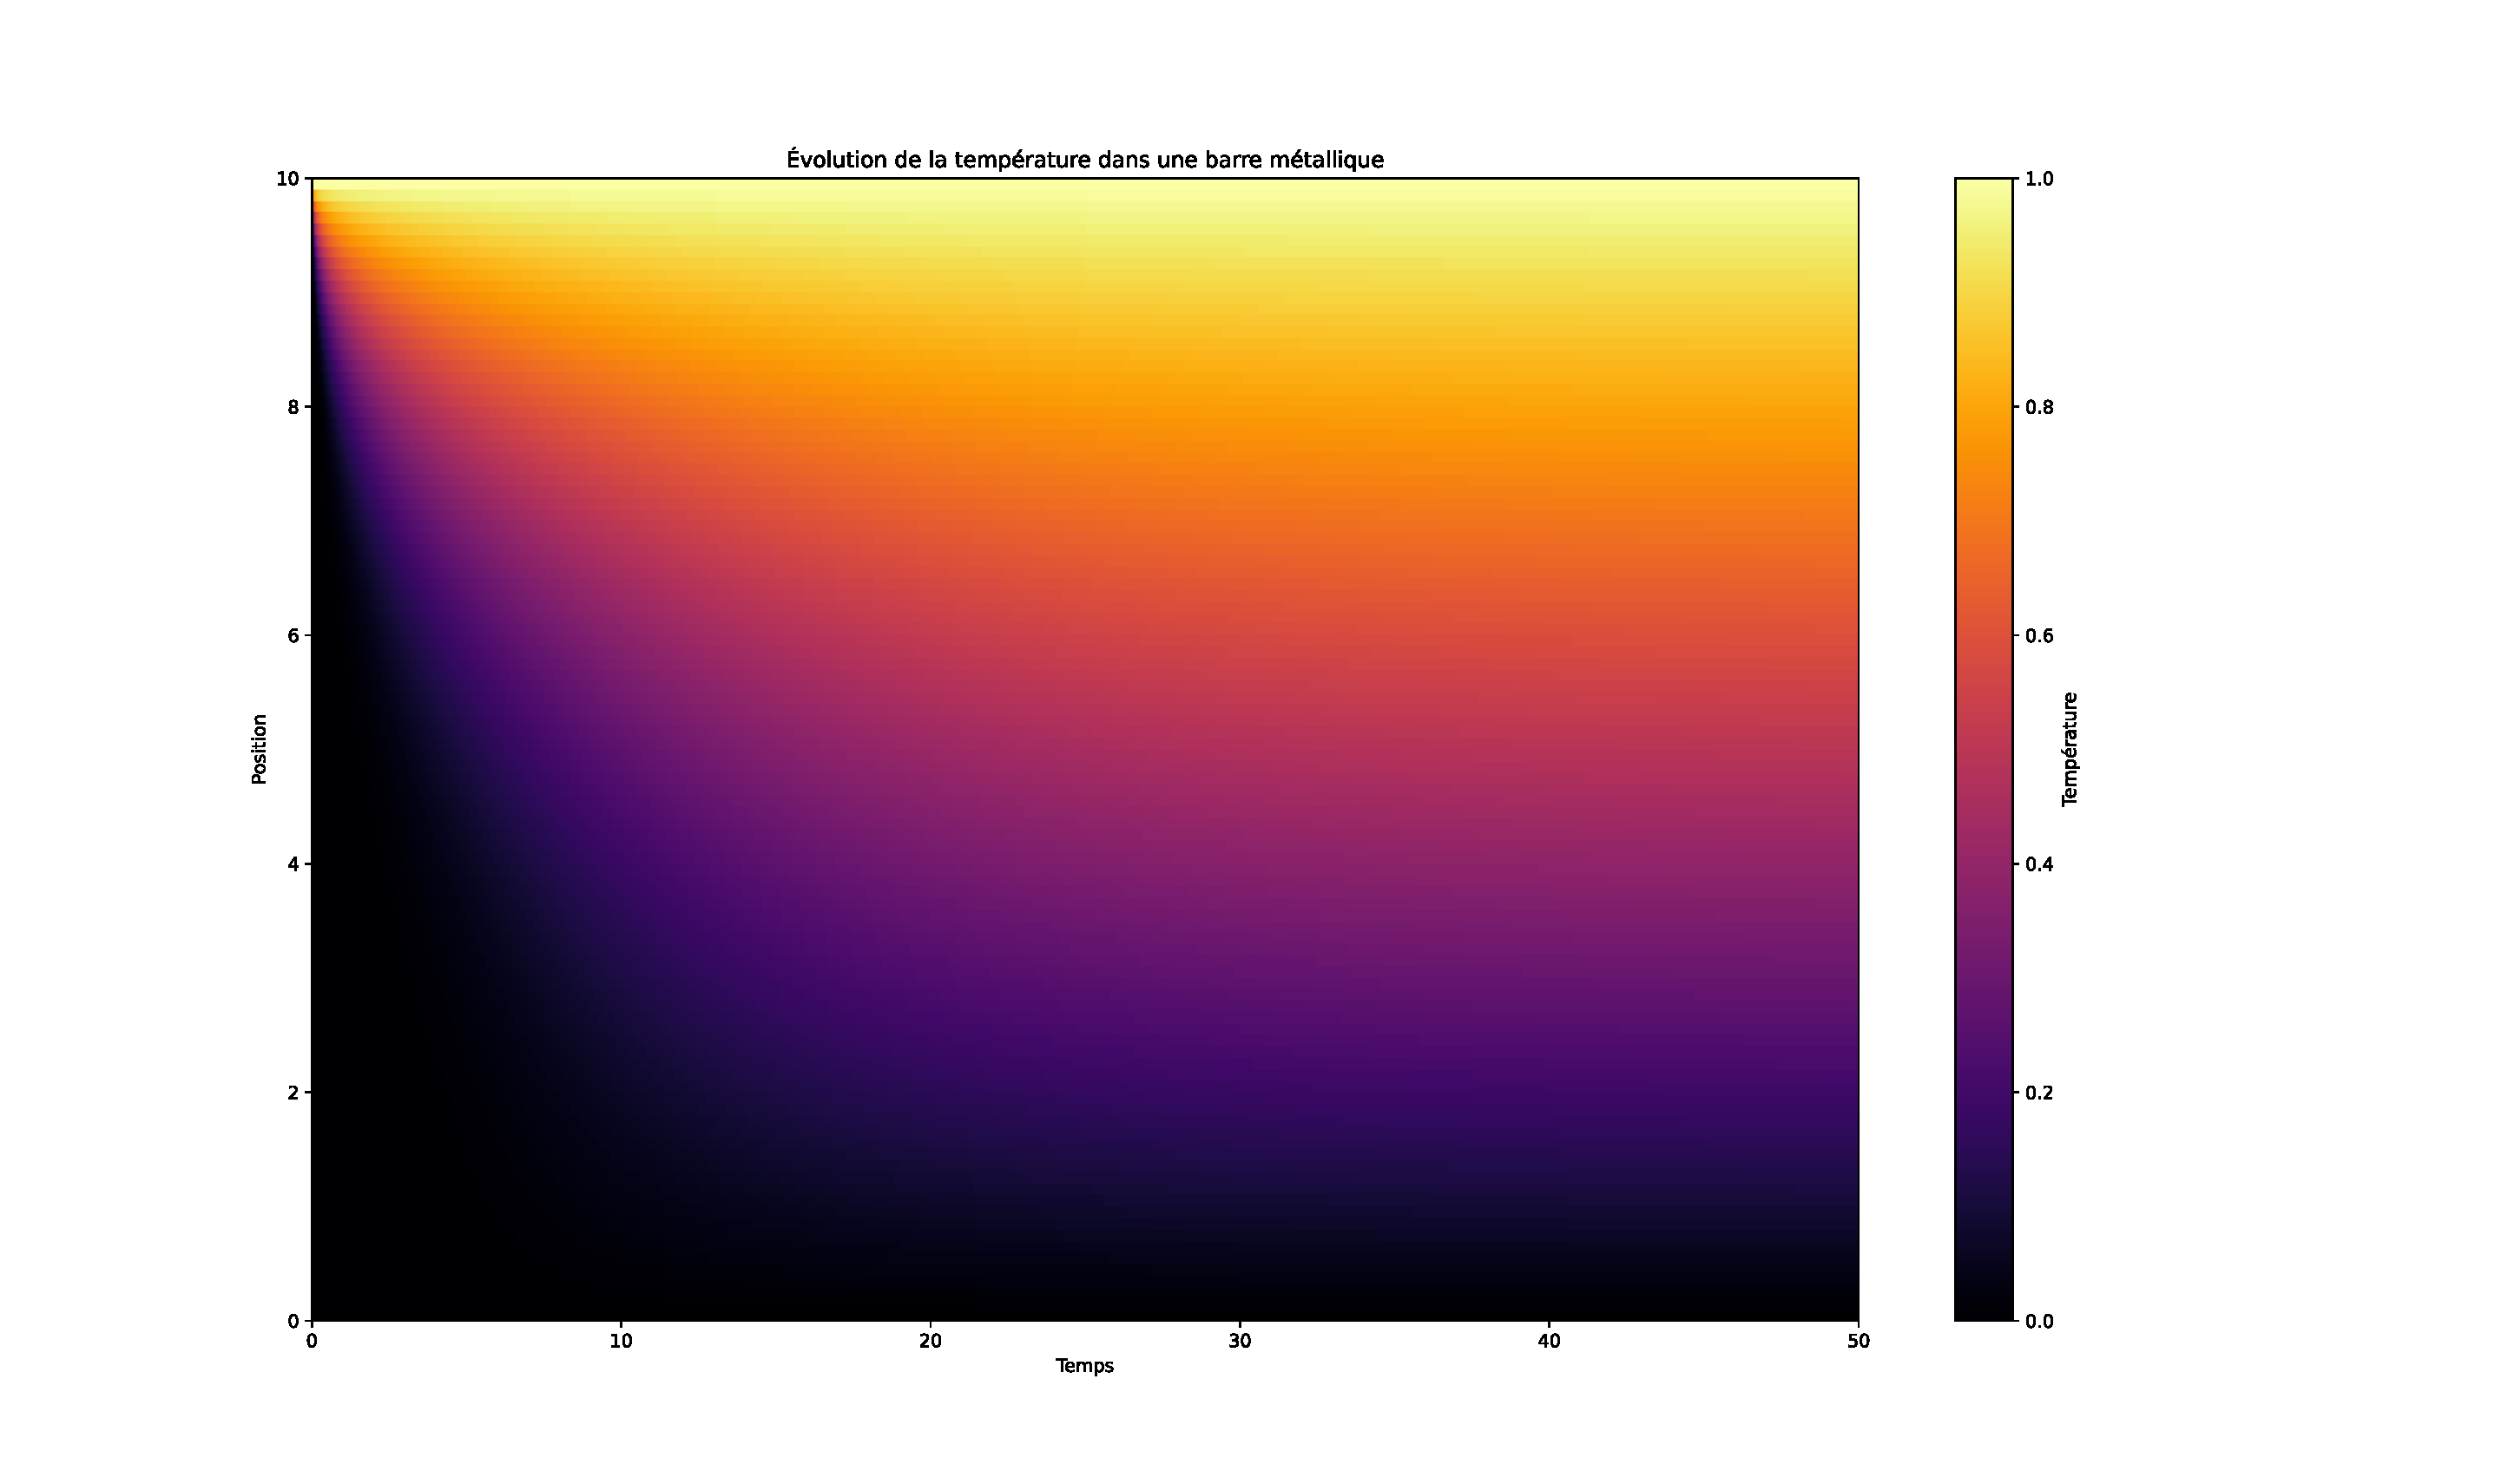
\includegraphics[width=1.2\linewidth]{figs/Figure_1.pdf}
    \end{center}


    \end{frame}


    \begin{frame}
    \frametitle{Résultats}
    \framesubtitle{Profil initial linéaire}

    \begin{center}
    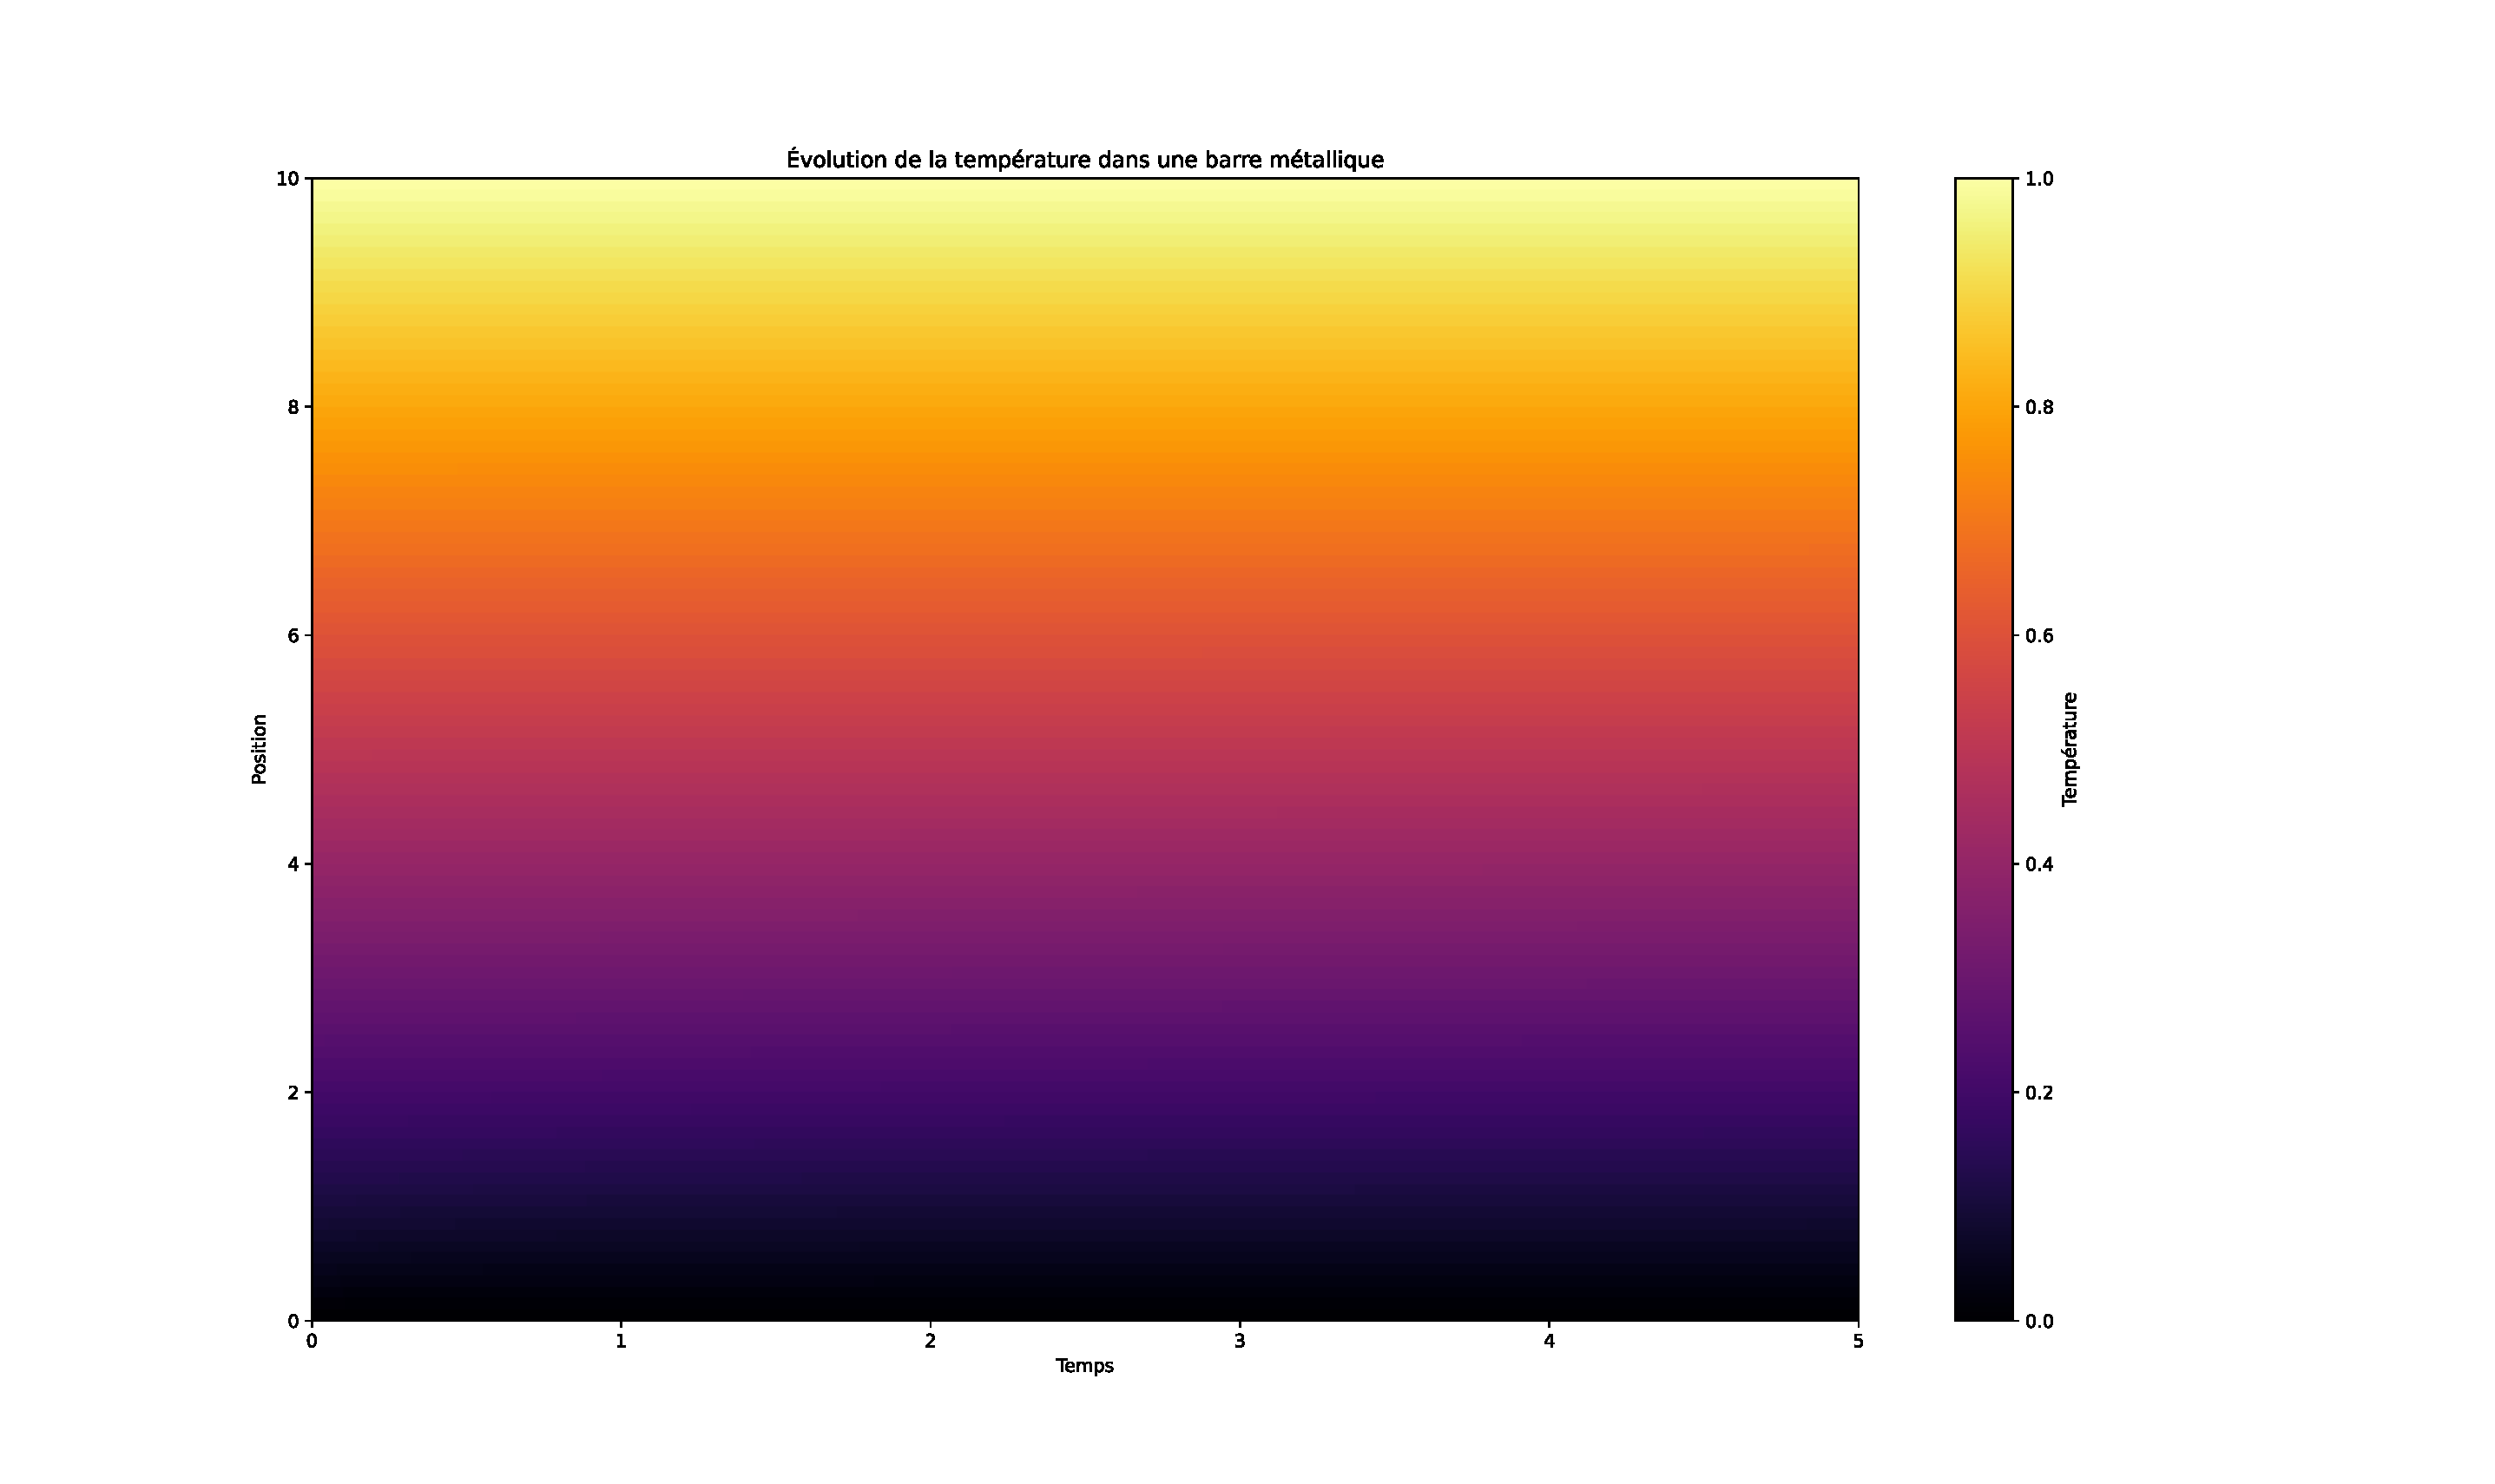
\includegraphics[width=1.2\linewidth]{figs/Figure_4.pdf}
    \end{center}


    \end{frame}


    \begin{frame}
    \frametitle{Résultats}
    \framesubtitle{Profil initial linéaire "inversé"}

    \begin{center}
    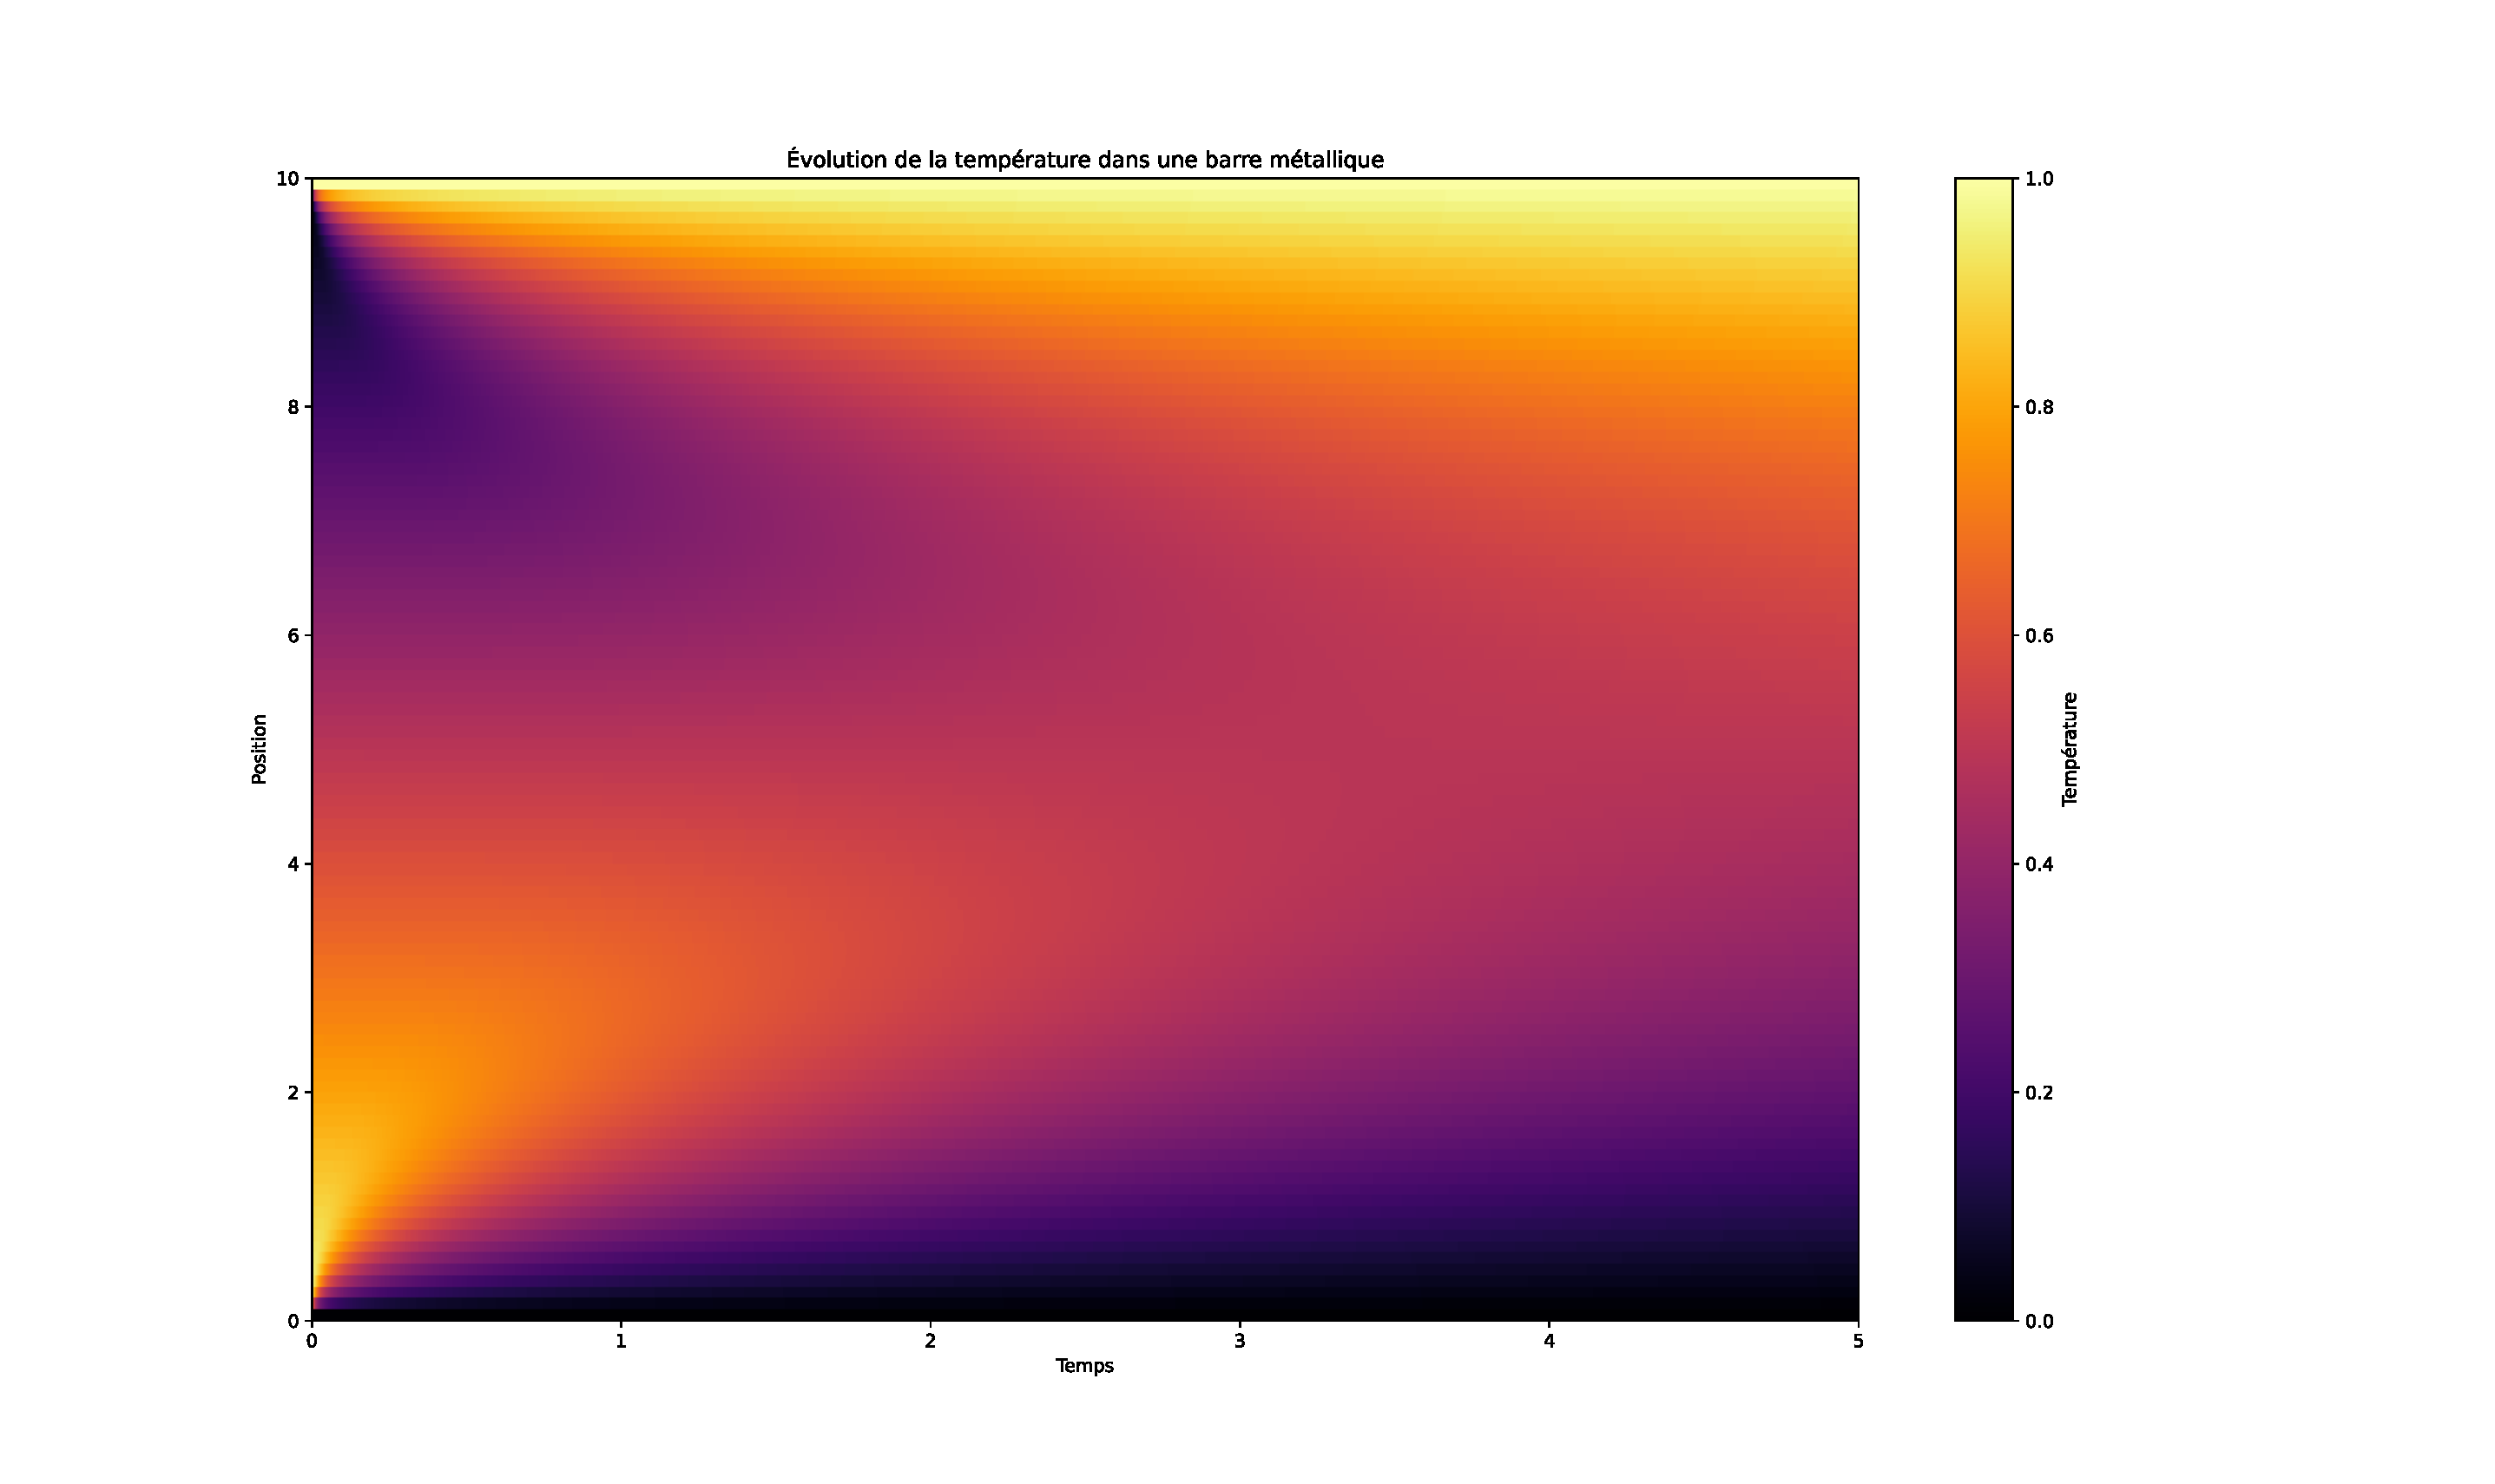
\includegraphics[width=1.2\linewidth]{figs/Figure_5.pdf}
    \end{center}


    \end{frame}



    \begin{frame}
    \frametitle{Résultats}
    \framesubtitle{Profil initial uniforme en $0.5$}

    \begin{center}
    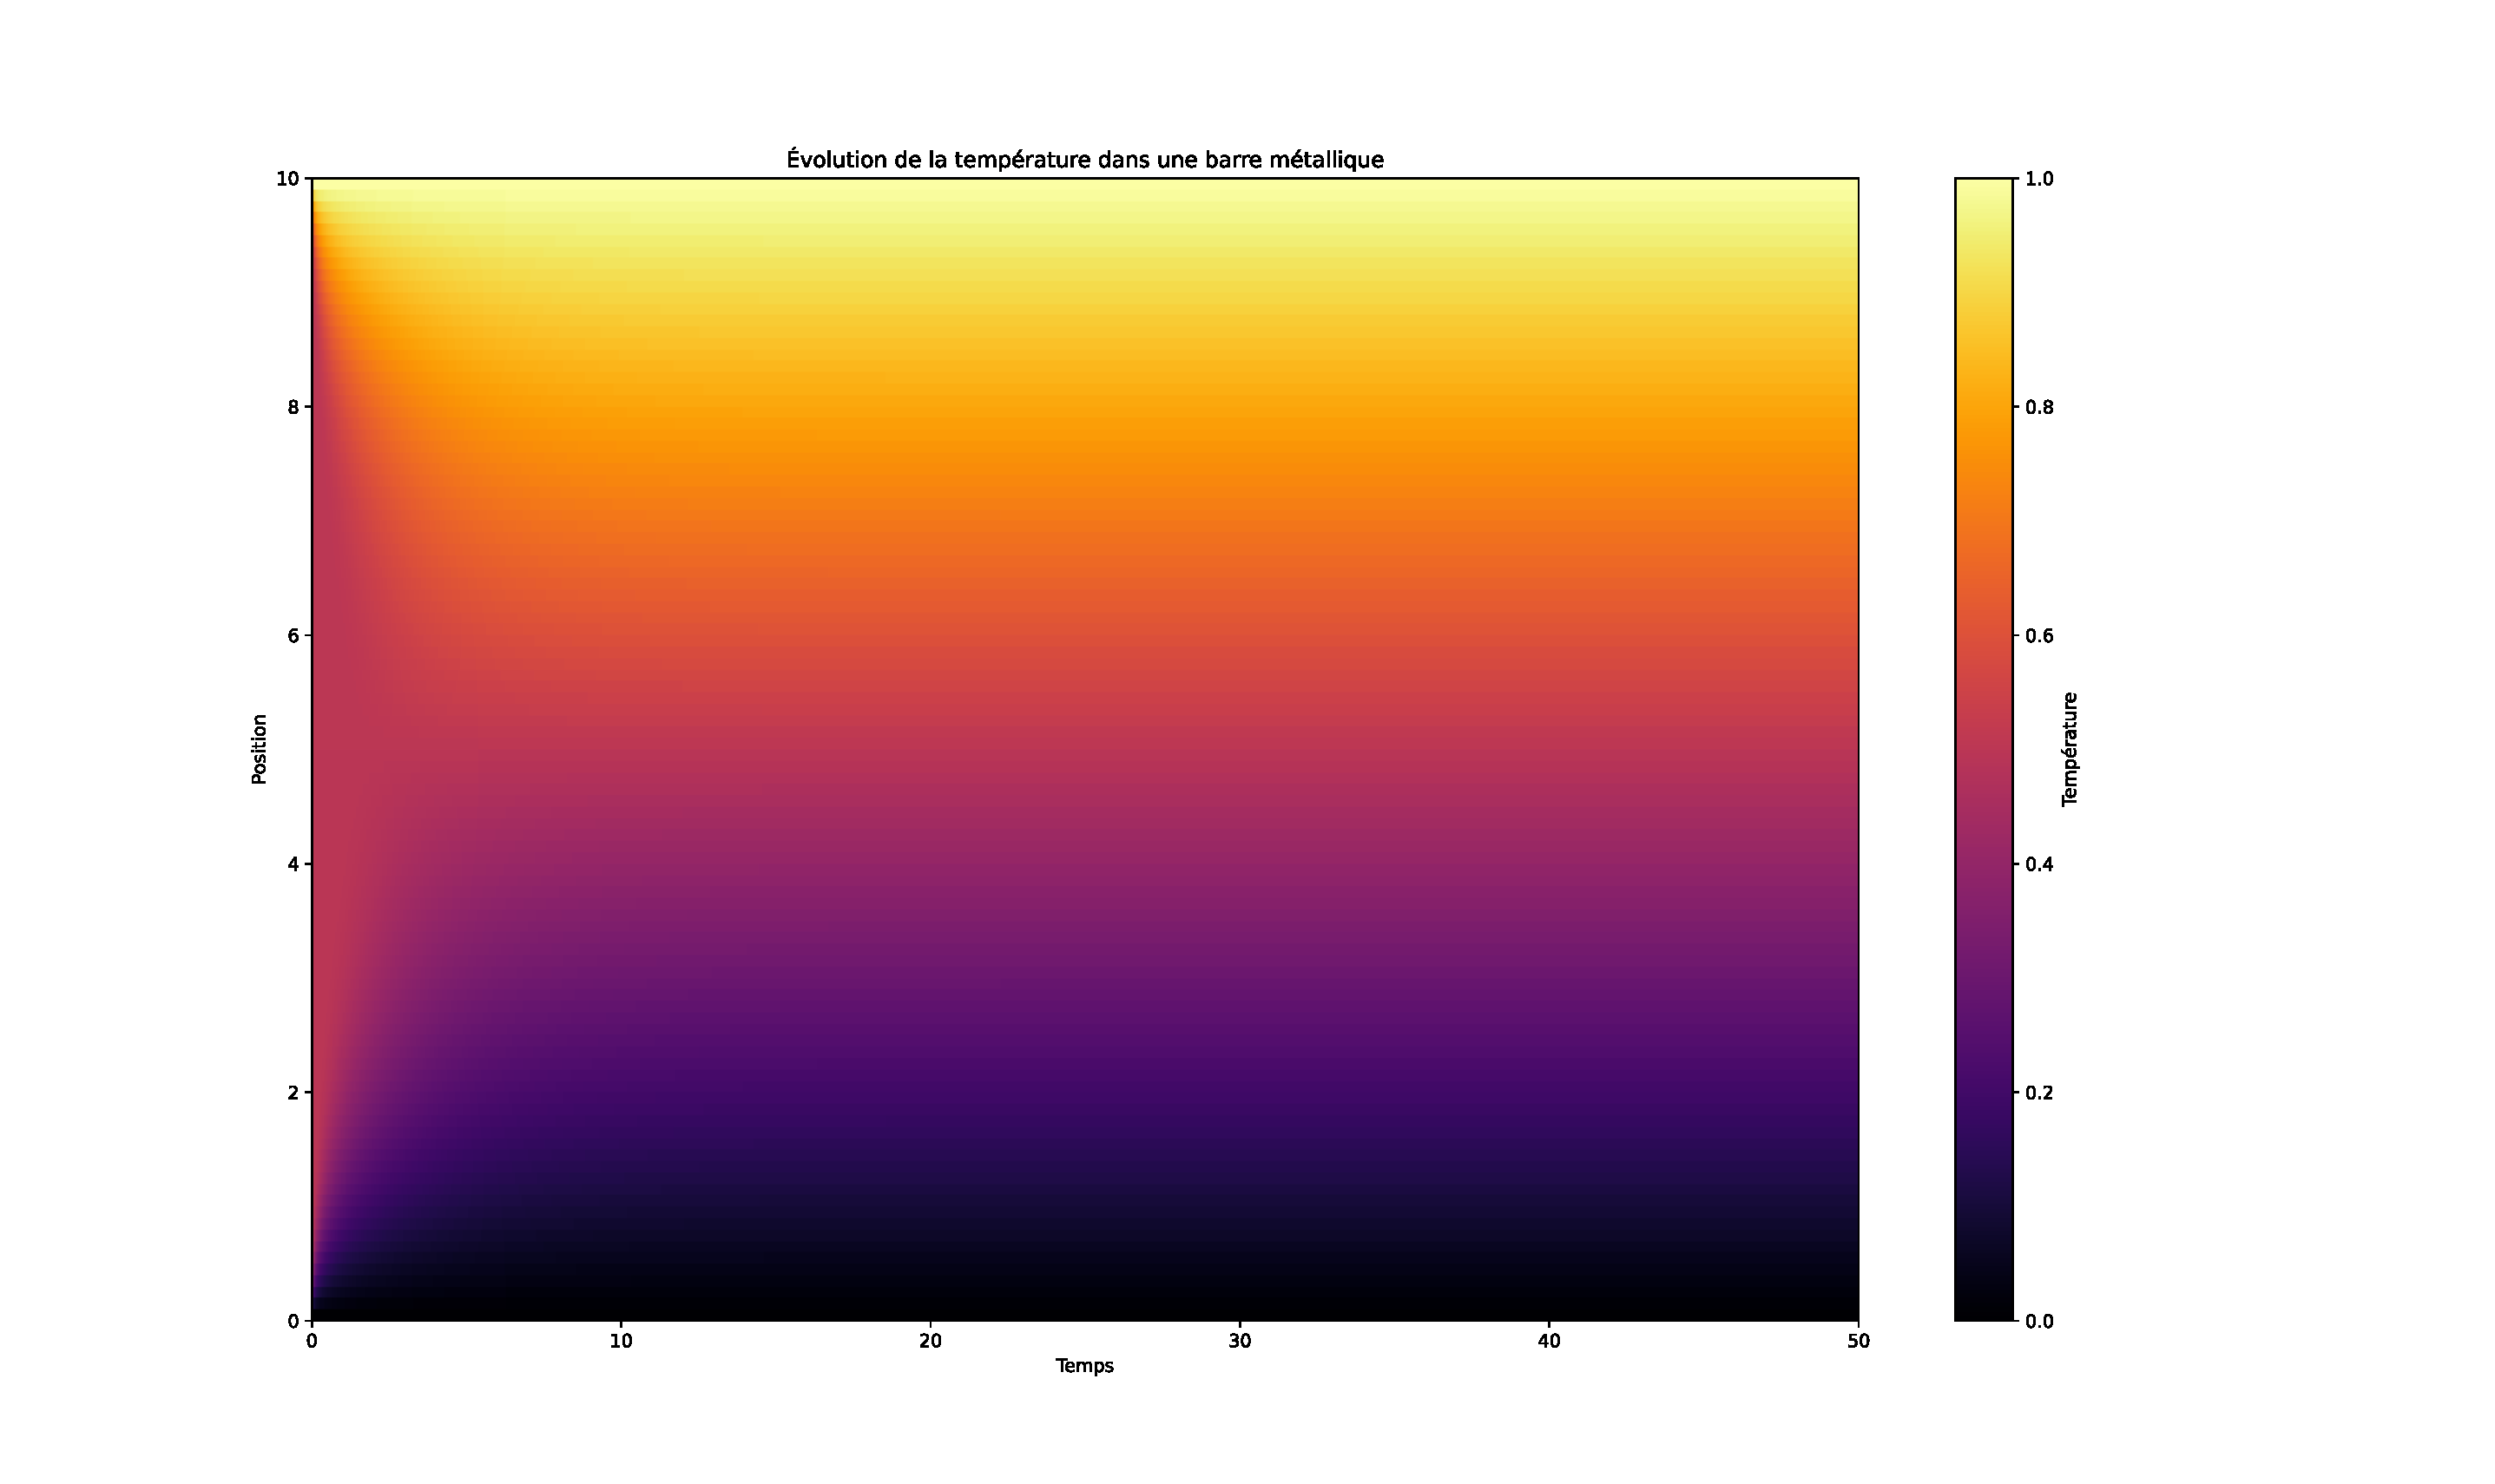
\includegraphics[width=1.2\linewidth]{figs/Figure_2.pdf}
    \end{center}


    \end{frame}

    \begin{frame}
    \frametitle{Résultats}
    \framesubtitle{Profil initial sinusoïdal (2 périodes, tf=5)}

    \begin{center}
    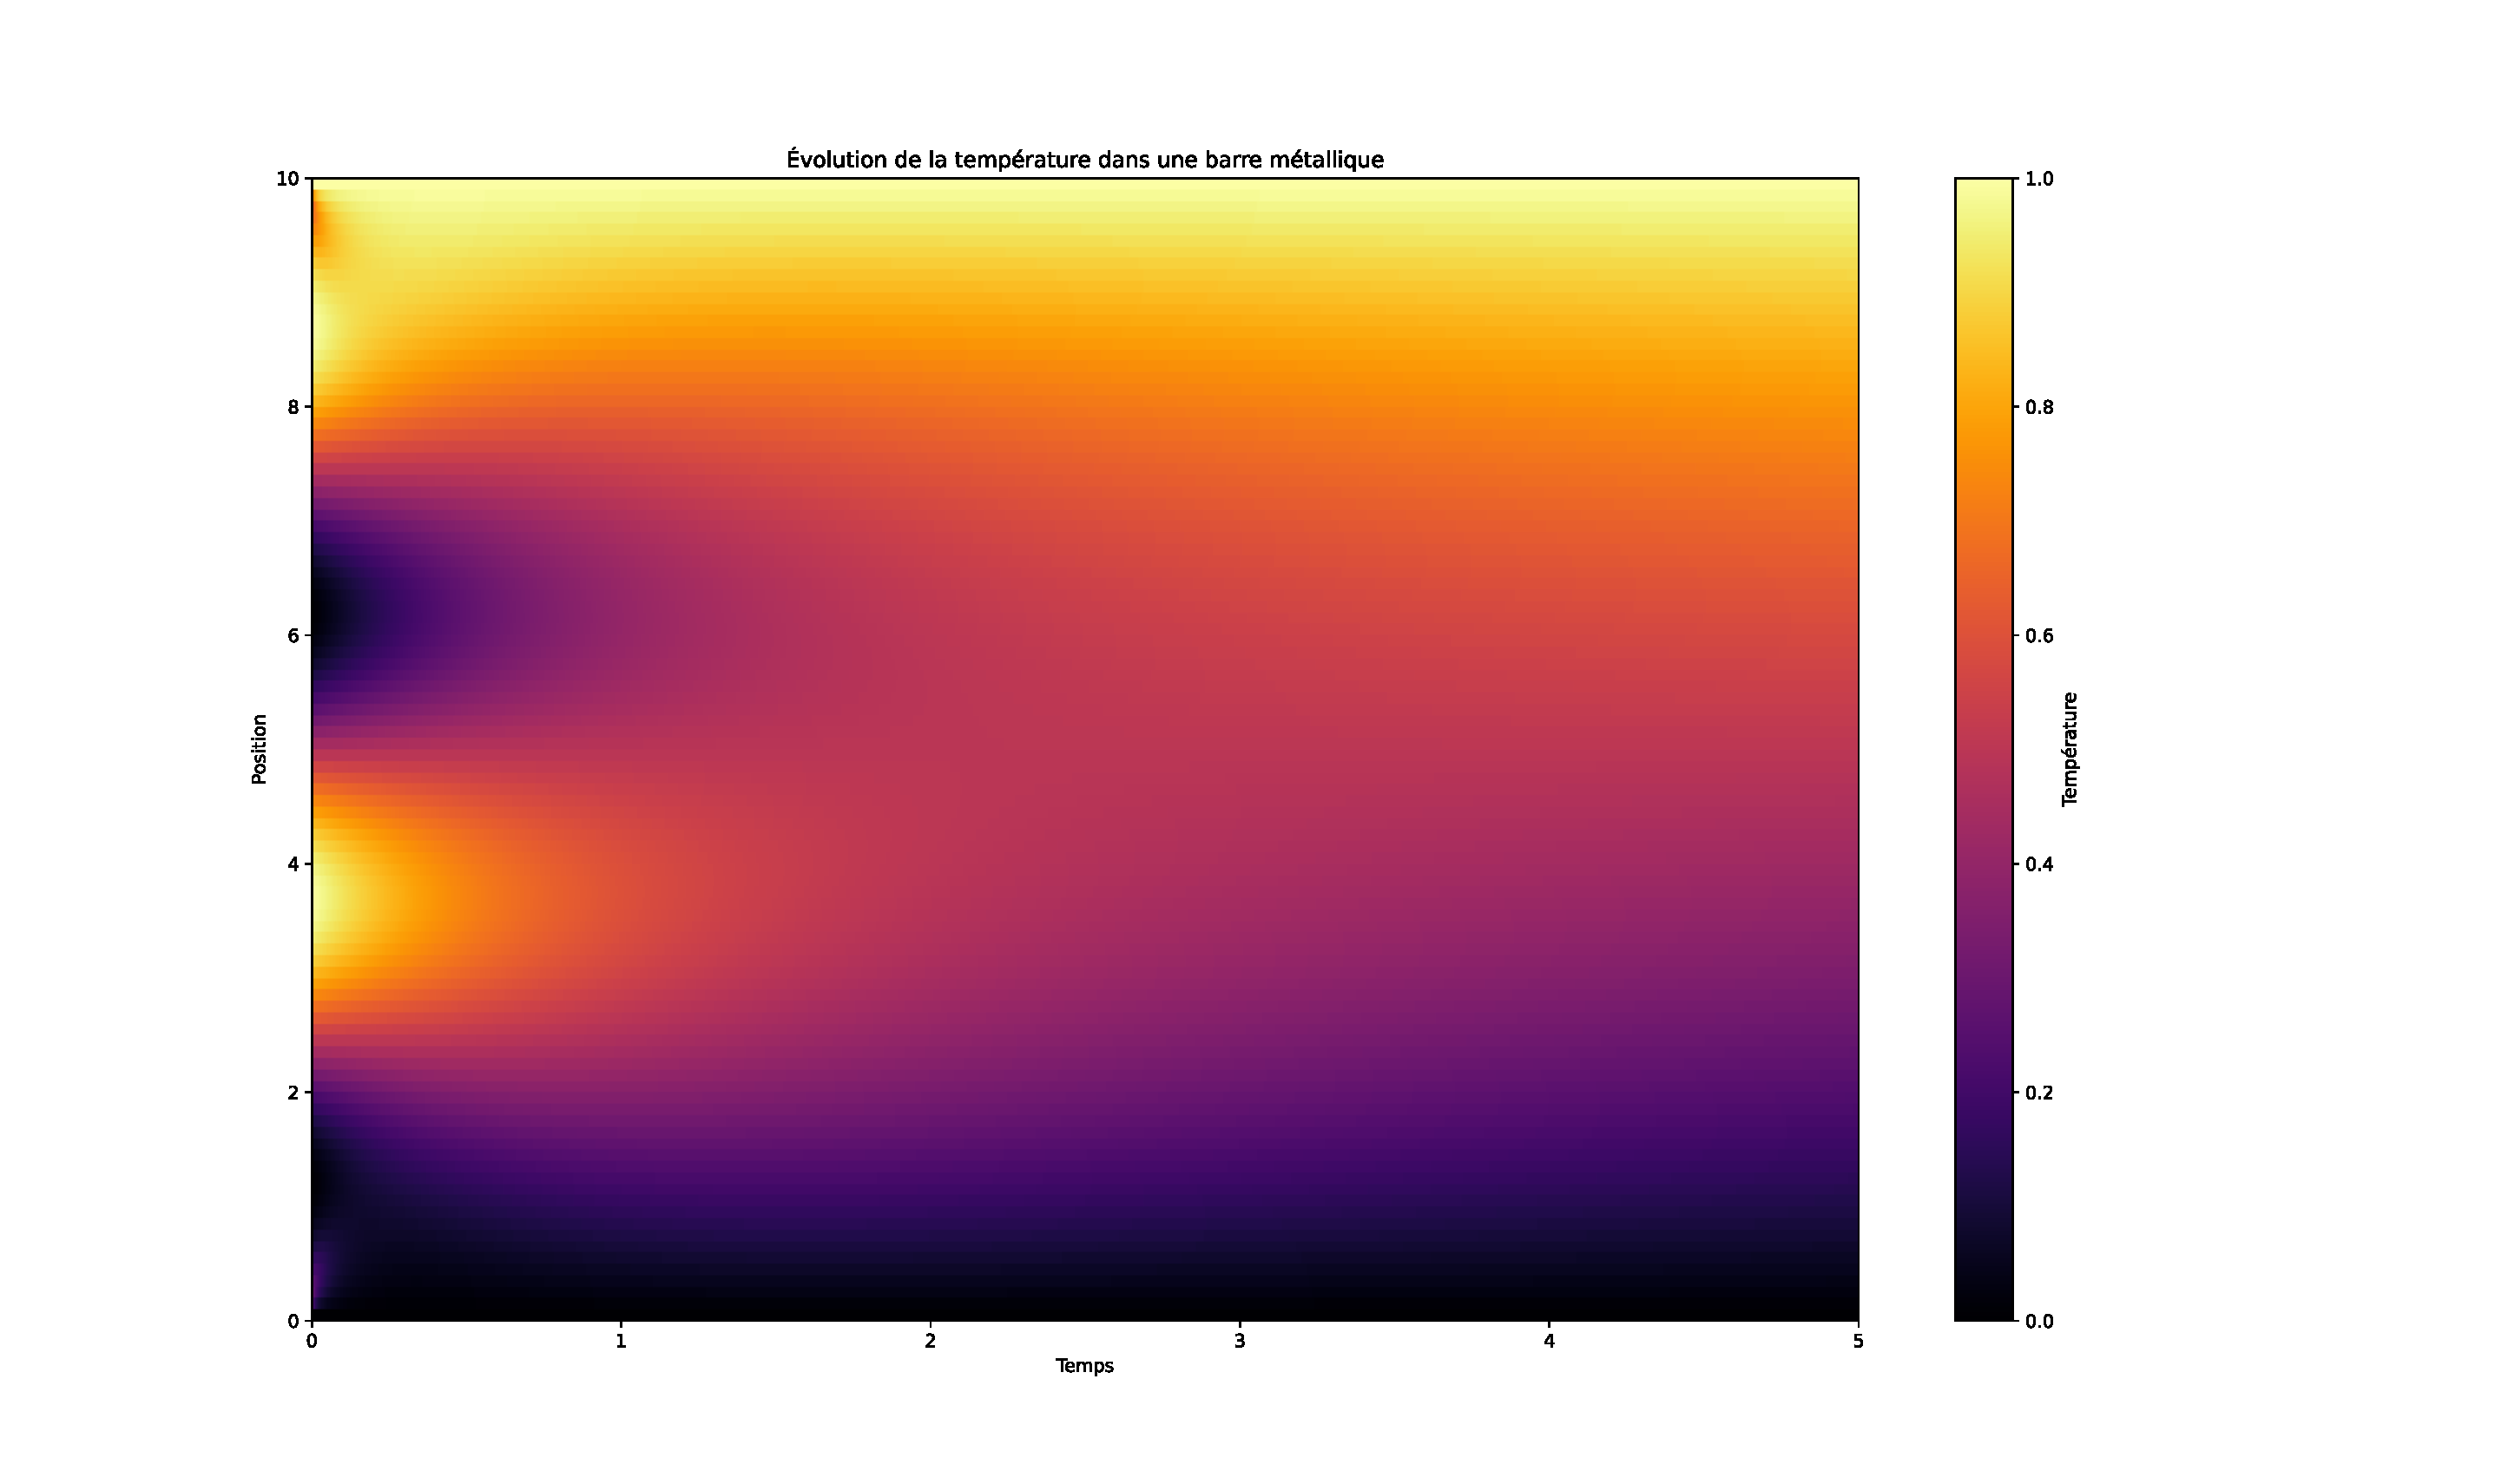
\includegraphics[width=1.2\linewidth]{figs/Figure_3.pdf}
    \end{center}


    \end{frame}











\end{document}
